\documentclass{article}
\usepackage[margin=0.1in]{geometry}
\usepackage{graphicx}

\begin{document}

\begin{table}
\centering
\resizebox{\textwidth}{!}{%
\begin{tabular}{|c|c|c|c|c|c|c|c|c|c|c|c|c|}
\hline & \multicolumn{4}{|c|}{\textbf{XGBoost}} & \multicolumn{4}{|c|}{\textbf{CN2}} & \multicolumn{4}{|c|}{\textbf{inTrees}} \\ \hline 
 & \textbf{acc} & \textbf{balacc} & \textbf{nodes} & \textbf{time} & \textbf{acc} & \textbf{balacc} & \textbf{nodes} & \textbf{time} & \textbf{acc} & \textbf{balacc} & \textbf{nodes} & \textbf{time} \\ \hline 
\textbf{wisconsinBreast}  & 0.9642+0.01$\sigma$ & 0.9609+0.01$\sigma$ & 550.3333+355.19$\sigma$ & 0.0894+0.04$\sigma$ & 0.9498+0.02$\sigma$ & 0.943+0.02$\sigma$ & 16.0+2.94$\sigma$ & 0.2099+0.1$\sigma$ & 0.9513+0.02$\sigma$ & 0.9461+0.02$\sigma$ & 12.3333+0.94$\sigma$ & 43.7857+4.54$\sigma$ \\ \hline 
\end{tabular}}
\end{table}

\begin{table}
\centering
\resizebox{\textwidth}{!}{%
\begin{tabular}{|c|c|c|c|c|c|c|c|c|c|c|c|c|}
\hline & \multicolumn{4}{|c|}{\textbf{QUESTGilles}} & \multicolumn{4}{|c|}{\textbf{CART}} & \multicolumn{4}{|c|}{\textbf{QUESTLoh}} \\ \hline 
 & \textbf{acc} & \textbf{balacc} & \textbf{nodes} & \textbf{time} & \textbf{acc} & \textbf{balacc} & \textbf{nodes} & \textbf{time} & \textbf{acc} & \textbf{balacc} & \textbf{nodes} & \textbf{time} \\ \hline 
\textbf{wisconsinBreast}  & 0.9484+0.01$\sigma$ & 0.941+0.01$\sigma$ & 23.6667+2.49$\sigma$ & 0.669+0.13$\sigma$ & 0.9413+0.01$\sigma$ & 0.9374+0.02$\sigma$ & 23.0+14.14$\sigma$ & 0.0018+0.0$\sigma$ & 0.9499+0.01$\sigma$ & 0.9499+0.0$\sigma$ & 8.3333+0.94$\sigma$ & 0.251+0.02$\sigma$ \\ \hline 
\end{tabular}}
\end{table}

\begin{table}
\centering
\resizebox{\textwidth}{!}{%
\begin{tabular}{|c|c|c|c|c|c|c|c|c|c|c|c|c|}
\hline & \multicolumn{4}{|c|}{\textbf{Genetic}} & \multicolumn{4}{|c|}{\textbf{RF}} & \multicolumn{4}{|c|}{\textbf{ISM_pruned}} \\ \hline 
 & \textbf{acc} & \textbf{balacc} & \textbf{nodes} & \textbf{time} & \textbf{acc} & \textbf{balacc} & \textbf{nodes} & \textbf{time} & \textbf{acc} & \textbf{balacc} & \textbf{nodes} & \textbf{time} \\ \hline 
\textbf{wisconsinBreast}  & 0.9484+0.01$\sigma$ & 0.9409+0.02$\sigma$ & 23.6667+4.71$\sigma$ & 703.5566+178.9$\sigma$ & 0.9628+0.01$\sigma$ & 0.9588+0.01$\sigma$ & 564.3333+333.14$\sigma$ & 1.6687+0.88$\sigma$ & 0.9484+0.0$\sigma$ & 0.9498+0.01$\sigma$ & 57.6667+33.48$\sigma$ & 87.6652+11.07$\sigma$ \\ \hline 
\end{tabular}}
\end{table}

\begin{table}
\centering
\resizebox{\textwidth}{!}{%
\begin{tabular}{|c|c|c|c|c|c|c|c|c|c|c|c|c|}
\hline & \multicolumn{4}{|c|}{\textbf{C4.5}} & \multicolumn{4}{|c|}{\textbf{GUIDE}} & \multicolumn{4}{|c|}{\textbf{ISM}} \\ \hline 
 & \textbf{acc} & \textbf{balacc} & \textbf{nodes} & \textbf{time} & \textbf{acc} & \textbf{balacc} & \textbf{nodes} & \textbf{time} & \textbf{acc} & \textbf{balacc} & \textbf{nodes} & \textbf{time} \\ \hline 
\textbf{wisconsinBreast}  & 0.9441+0.01$\sigma$ & 0.9337+0.02$\sigma$ & 18.3333+4.99$\sigma$ & 0.0075+0.0$\sigma$ & 0.937+0.01$\sigma$ & 0.9274+0.01$\sigma$ & 11.6667+0.94$\sigma$ & 0.2603+0.03$\sigma$ & 0.9427+0.0$\sigma$ & 0.9415+0.01$\sigma$ & 117.0+5.89$\sigma$ & 65.6779+11.17$\sigma$ \\ \hline 
\end{tabular}}
\end{table}

\begin{figure}\centering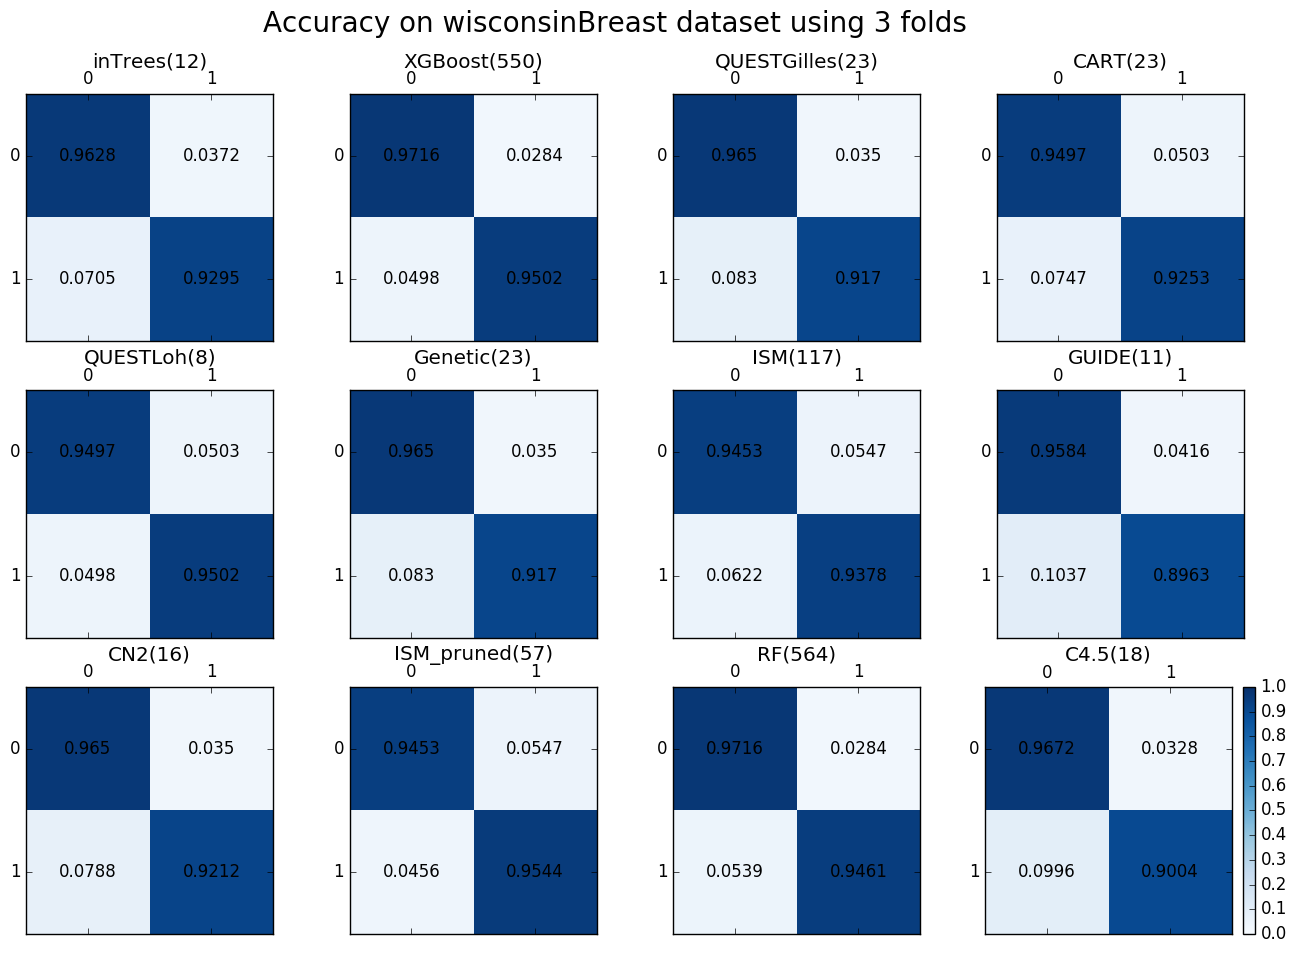
\includegraphics[width=\textwidth]{wisconsinBreast_CV3genetic3109.png}\caption{Confusion matrix for wisconsinBreast}\end{figure}
\end{document}